\subsection{Dalvik Executionable File Format} \label{subsection:android-dex}
\begin{itemize}
    \item android uses dex, executed by dvm
    \item compiled from java bytecode
    \item different, stack vs register for arm
    \item direct mapping from code to registers, uses 32 bit register, 64 bit use adjacent registers
    \item bitcode less compact, 16 bit instead of 8bit in java
    \item 218 opcodes, dest source ordering
    \item in java heterogenous pools, dx for dalvik merges, reduce dublicates, best for strings
    \item all classes into one file as well
    \item optimization, dex odex same semantics
    \item downside, easy to reverse engineer
\end{itemize}
\begin{figure}[h]
    \centering
    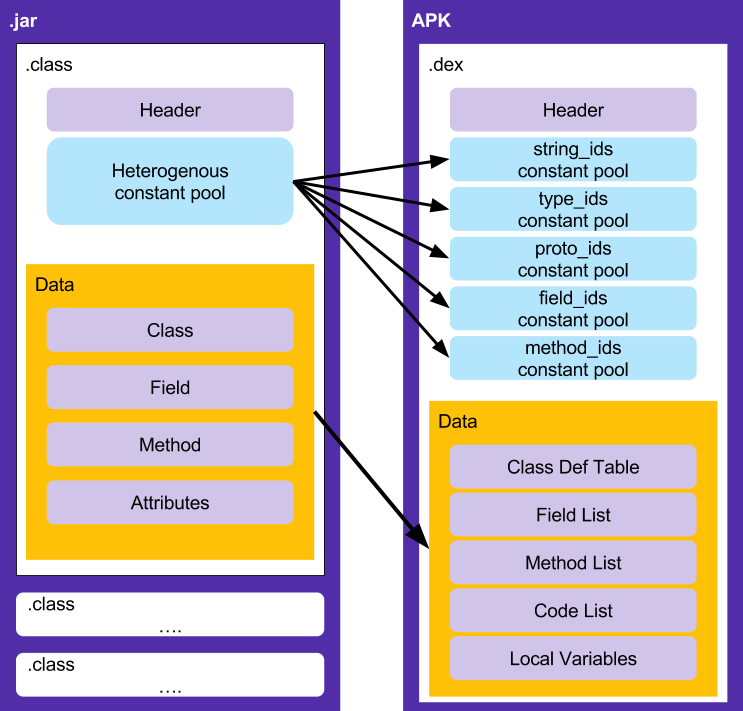
\includegraphics[width=0.5\textwidth]{data/java.png}
    \caption{\gls{jar} to \gls{apk} transformation \cite{googleDalvik}}
    \label{fig:java}
\end{figure}

\begin{figure}[h]
    \centering
    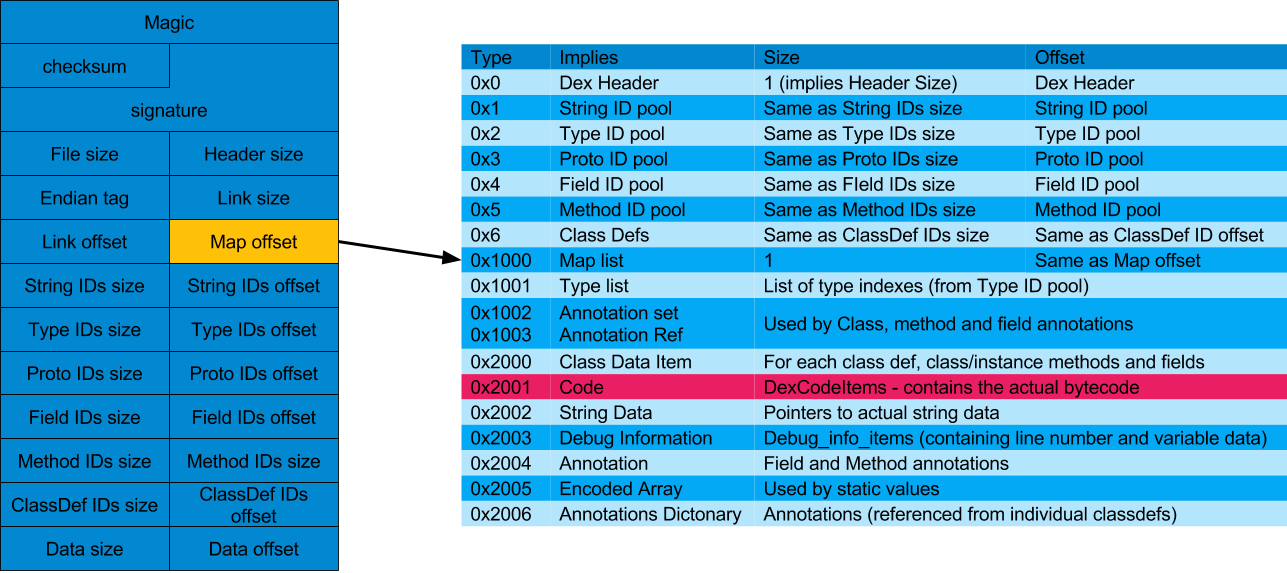
\includegraphics[width=0.8\textwidth]{data/dex.png}
    \caption{\gls{dex} file format \cite{andevconDalvikART}}
    \label{fig:dex}
\end{figure}
